\documentclass[dvisvgm]{standalone}

\usepackage{tikz}
\usetikzlibrary {arrows.meta,automata,positioning}

\begin{document}

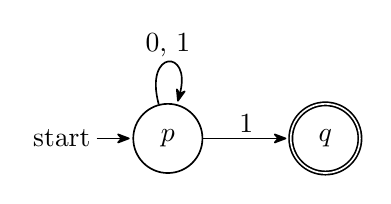
\begin{tikzpicture}[->,>={Stealth[round]},shorten >=1pt,%
    auto,node distance=2cm,on grid,semithick,
    inner sep=2pt,bend angle=45]

    \node[initial,   state] (A)              {$p$};
    \node[accepting, state] (B) [right=of A] {$q$};

    \path [->]
        (A) edge              node {1}     (B)
        (A) edge [loop above] node {0, 1}  (A);
\end{tikzpicture}

\end{document}